\TChapter{Avances}{epsilon}
\ \\\\
En esta sección se mostrarán los avances que hasta el día de hoy se tienen.

\section{Herramientas utilizadas}
Para el desarrollo de los avances para el presente trabajo se utilizó el lenguaje de programación Python, se utilizó Anaconda debido a que
es una distribucion de Python que se utiliza para el análisis de datos, es decir con Anaconda tenemos un ambiente de trabajo para el análisis 
de datos. Mientras que para el web- crawling se utilizó Scrapy, el cual es un framework que nos permite el web scraping para la extracción de 
información de los sitios web.

\section{Estudio previo}
Una vez que se eligieron las herramientas que nos iban a proporcionar la información de las páginas web, se procedió con el estudió de los 
sitios de los cuales se extraerían noticias para el entrenamiento.

En primera instancia se eligiero 9 sitios web (\ref{tabla:sitios}):

\begin{itemize}
    \item 3 Sitios de foros de noticias: Aristegui Noticias, SDP Noticias y Sopitas.
    \item 3 Sitios de diarios: El Universal, La Jornada y Excelsior.
    \item 3 Sitios televisivos: TV Azteca, Televisa y Once Noticias.
\end{itemize}


\begin{table}[htbp]
    \centering
    \resizebox{\columnwidth}{!}{%
    \begin{tabular}{r|l|l|l|l|l|l|l|l|l|}
    \multicolumn{1}{r}{Sección}
    & \multicolumn{1}{l}{El Universa1}
    & \multicolumn{1}{l}{La Jornada}
    & \multicolumn{1}{l}{Excelsior} 
    & \multicolumn{1}{l}{Aristegui Noticias} 
    & \multicolumn{1}{l}{SDP Noticias} 
    & \multicolumn{1}{l}{Sopitas} 
    & \multicolumn{1}{l}{Azteca Noticias} 
    & \multicolumn{1}{l}{Televisa} 
    & \multicolumn{1}{l}{Once Noticias} \\ \cline{2-10}
        Nacional & Nacional      & -            & Nacional      & México                & Nacional      & Noticias  & -                 & Nacional      & Nacional      \\ \hline
        Internacional & Mundo    & Mundo        & Global        & Destacado/Mundo       & Internacional & -         & Internacional     & Internacional & Internacional \\ \hline
        Ciudad   & Metrópoli     & Capital      & Comunidad     & -                     & CDMX          & -         & -                 & CDMX          & CDMX      \\ \hline
        Estados  & Estados       & Estados      & Estados       & Sociedad/México       & Locales       & -         & Estados           & Estados       & Nacional   \\ \hline
        Economía & Cartera       & Economía     & Dinero        & Economía              & Economía      & -         & Finanzas          & Economía      & Economía   \\ \hline
        Deportes & Deportes      & Deportes     & Adrenalina    & Deportes              & Deportes      & Deportes  & -                 & Deportes      & Deportes   \\ \hline
        Espectáculos & Espectáculos & Espectáculos & Función    & -                     & En el show    & Entretenimiento & -           & Espectáculos  & Deportes    \\ \hline
        Cultura  & Cultura       & Cultura      & -             & -                     & -             & -         & -                 & Arte y cultura & Cultura   \\ \hline
        Política & -             & Política     & Política      & Poderes               & -             & -         & Política          & Política      & -   \\ \hline
\end{tabular}%
\label{tabla:sitios}
}
\end{table}

Una vez que se analizarón las secciones con las que contaba cada sitio se procedió a homologar las secciones en las cuales la mayoría de los 
sitios coincidian, por lo cual se quedarón definidas 5 secciones para clasificación de las noticias extraídas.

\begin{itemize}
    \item Política
    \item Deportes
    \item Ciencia y tecnología
    \item Economía
    \item Cultura
\end{itemize}

Posteriormente se procedio con la recolección de noticias. 
La biblioteca utilizada es Scrapy la cual nos servirá para el Scrapeo.

Una de las cosas que se debía investigar sobre cada sitio web fue su estructura XML, al saber la estructura del contenido de una página  
nos permite realizar el Scrapeo de manera correcta y eso depende de cada sitio, ya que no todos los sitios cuentan con una página la cual tenga 
las mismas secciones o el mismo orden.
\\

\section{Recolección de noticias}

\subsection{Prerrequisitos}
\begin{itemize}
    \item Tener instalado en nuestro computador alguna versión de Linux.
    \item Tener instalado python en a partir de su versión 2.7
    \item Tener en cuenta que se necesitará utilizar entornos virtuales
\end{itemize}

Abriremos una terminal nueva con la ruta donde se desee guardar el proyecto, figura \textbf{\ref{fig:uno}} 

\begin{figure}[H]
  \centering
  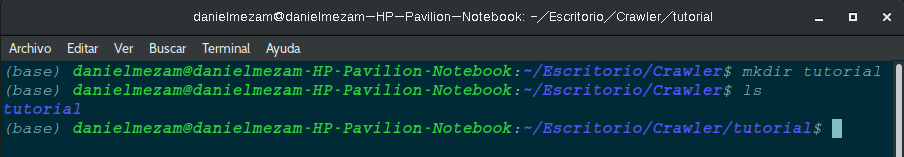
\includegraphics[scale=.35]{imagenes/Capitulo5/1}
  \caption{Carpeta donde se creará el proyecto.}
  \label{fig:uno}
\end{figure}

Una vez ubicados en la carpeta donde se creará el proyecto se procede con la creación de un entorno virtual y ahí se activará el entorno virtual 
creado figura \textbf{\ref{fig:dos}} .

\begin{figure}[H]
    \centering
    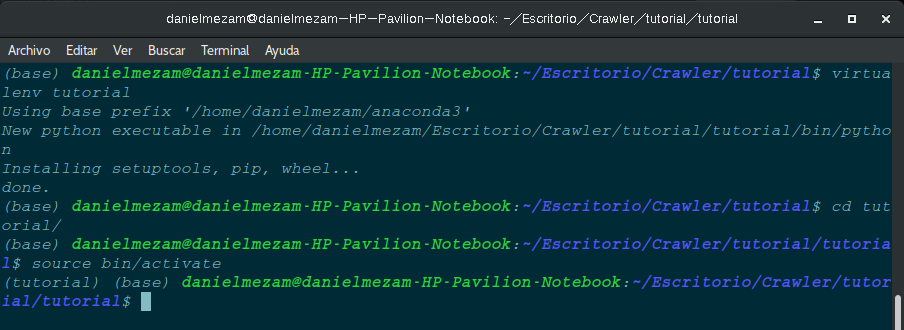
\includegraphics[scale=.35]{imagenes/Capitulo5/2}
    \caption{Creación del entorno virtual.}
    \label{fig:dos}
  \end{figure}

Una vez en nuestro entorno virtual instalaremos Scrapy y procederemos con la creación del proyecto con la siguiente línea
\textbf{\textit{scrapy startproject tutorial}} figura \textbf{\ref{fig:tres}} .

\begin{figure}[H]
    \centering
    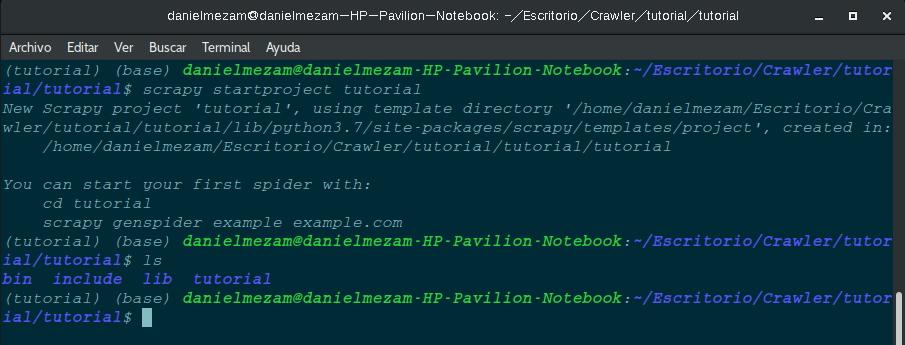
\includegraphics[scale=.35]{imagenes/Capitulo5/3}
    \caption{Creación del proyecto Scrapy.}
    \label{fig:tres}
  \end{figure}

Veremos que se ha creado una carpeta con el nombre del proyecto \textbf{"tutorial"} la cual contiene los siguientes archivos figura \textbf{\ref{fig:cuatro}} .

\begin{figure}[H]
    \centering
    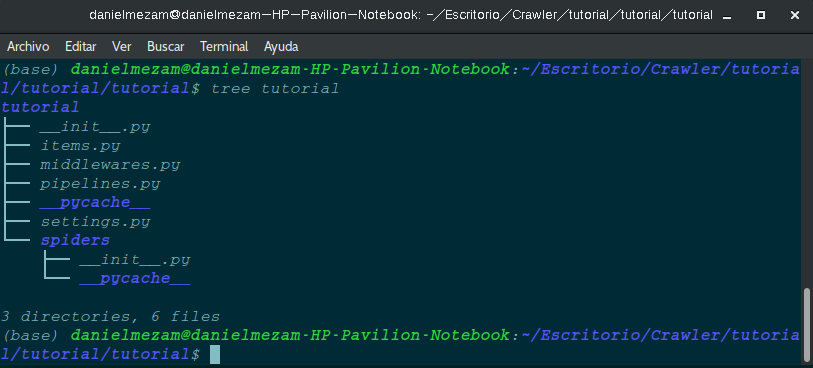
\includegraphics[scale=.35]{imagenes/Capitulo5/4}
    \caption{Carpetas y archivos creados.}
    \label{fig:cuatro}
  \end{figure}

Crearemos un archivo dentro de la carpeta Spiders llamado \textbf{\textit{spiders.py}} 
\\
Definimos las partes de la página que deseamos recolectar  de cada noticias y lo guardamos en el archivo \textbf{items.py}  \textbf{\ref{fig:cinco}}.
Para nuestro recolector es claro que necesitamos los siguientes aspectos de cada noticia, lo cual nos permitirá obtener mejores resultados
\begin{itemize}
  \item URL: Se necesita la URL para redireccionar al usuario a la página de la noticia seleccionada.
  \item Sección: Necesitamos saber la sección para nuestro entrenador.
  \item Título: El título de la noticia permitirá al usuario saber sobre la noticia.
  \item Autor: Permitirá mostrarle al usuario el autor de la noticia.
  \item Fecha: Se necesitará la fecha para su clasificación por la fecha de publicación de la noticia.
  \item Descripción: Se mostrara al usuario una pequeña descripción de la noticia si es que la tiene.
  \item Noticia: La noticia nos ayudará a la clasificación de la misma.
\end{itemize}

\begin{figure}[H]
  \centering
  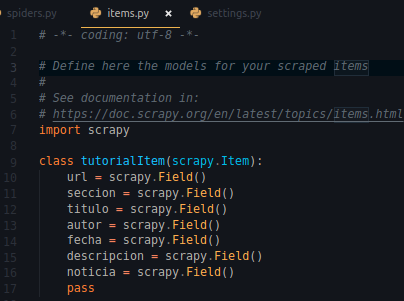
\includegraphics[scale=.45]{imagenes/Capitulo5/5}
  \caption{Secciones de la página que deseamos recolectar.}
  \label{fig:cinco}
\end{figure}

En el archivo spiders.py se definen las reglas que debe seguir el recolector \textbf{\ref{fig:seis}}

\begin{figure}[H]
  \centering
  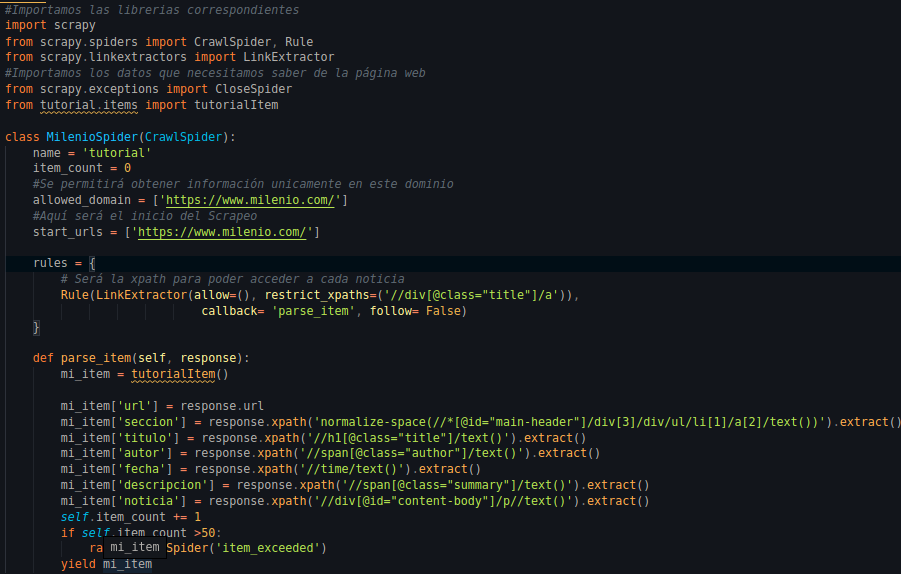
\includegraphics[scale=.45]{imagenes/Capitulo5/6}
  \caption{En la primera parte vemos las librerias, posteriormente se definen las reglas las cuales son diferentes para cada sitio web.}
  \label{fig:seis}
\end{figure}

Se debe considerar que se debe analizar la página para poder obtener los datos de la misma, y se debe ser muy específico, de lo contrario 
no se podrá recolectar de manera correcta la información.

Una vez definidas las reglas para la extracción se procede con la exportación del documento, en el cual se guardará la información recolectada.

Posteriormente se procede a modificar el archivo \textbf{pipelines.py} el cual cnos permitirá hacer la importación de la información obtenida a un 
archivo en formato CSV \textbf{\ref{fig:siete}}

\begin{figure}[H]
  \centering
  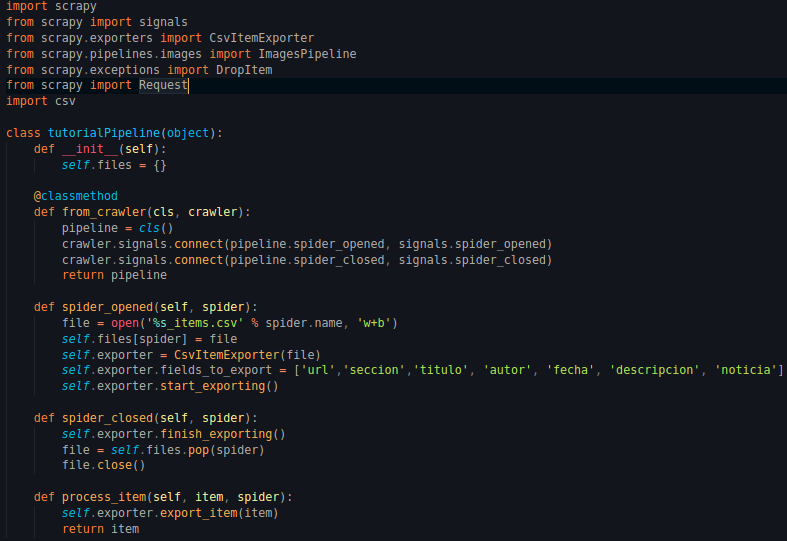
\includegraphics[scale=.45]{imagenes/Capitulo5/7}
  \caption{Código anexado para la exportación de la informacióne extraída.}
  \label{fig:siete}
\end{figure}

Por último se debe ejecutar el siguiente comando para extraer la información \textbf{scrapy crawl tutorial -t csv} \textbf{\ref{fig:ocho}}

\begin{figure}[H]
  \centering
  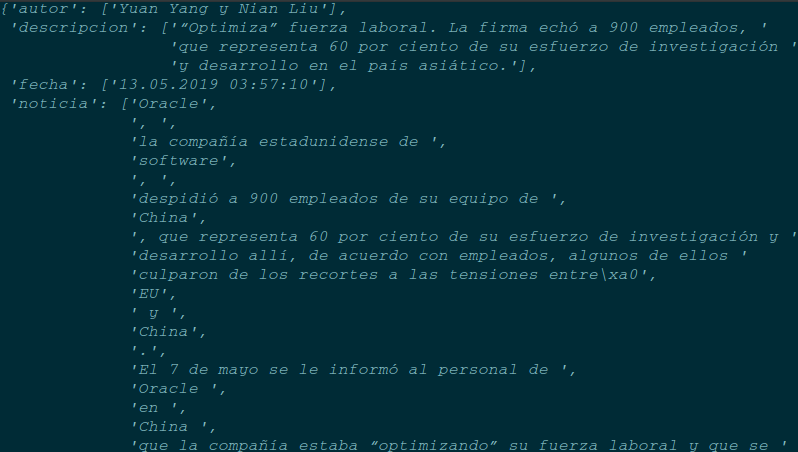
\includegraphics[scale=.35]{imagenes/Capitulo5/8}
  \caption{Muestra de la recolección por parte del crawler.}
  \label{fig:ocho}
\end{figure}

\subsection{Resultados}
Una vez que termino de ejecutarse el crawler se generó un archivo CSV, ahí se almaceno la información recolectada, posteriormente toda la información 
que se arecolectada será utilizada para el algoritmo de entrenamiento textbf{\ref{fig:nueve}}.

\begin{figure}[H]
  \centering
  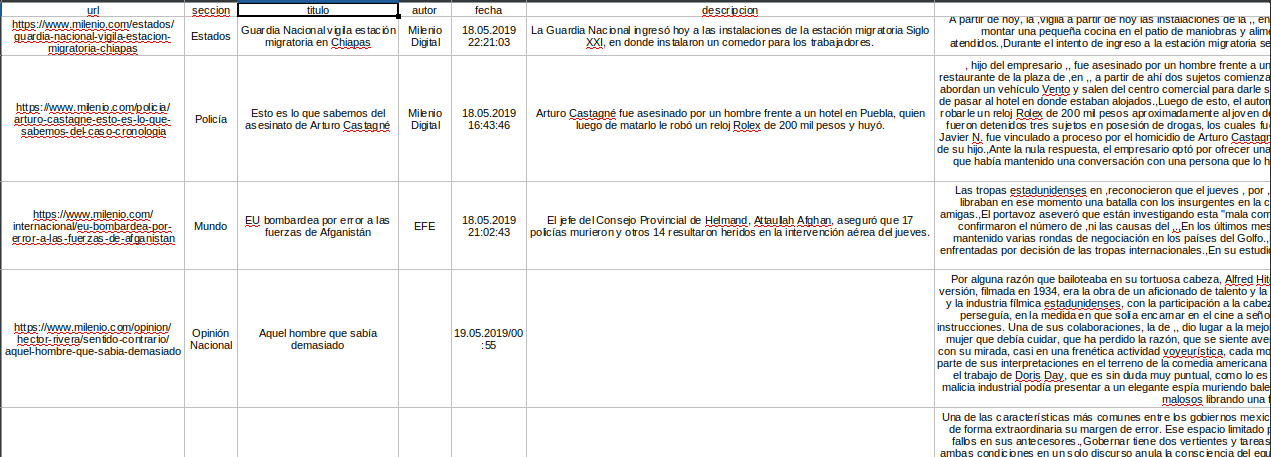
\includegraphics[scale=.35]{imagenes/Capitulo5/9}
  \caption{Resultados obtenidos dela extracción del sitio web almacenado en un archivo CSV.}
  \label{fig:nueve}
\end{figure}


\subsection{Consideraciones}
\begin{itemize}
  \item Se debe tener conocimiendo de XML para poder realizar las reglas que nos permitirán extraer información de la página web que solicitemos extraer 
  información y no se extraíga espacios en blanco.
  \item Cuando la noticia consta de un video, no se obtiene ninguna información adicional de la noticia.
  \item Se debe tomar en cuenta que las secciones no están homogeneizadas, es decir a pesar de que de la misma página existan varias secciones 
  \item La distribución de la información varia dependiendo a la sección y sitio web.
  \item Se acoto el periodo de busqueda de noticias ya que algunos sitios web muestran las noticias más recientes, lo cual no nos permite realizar 
  el trabajo del Crawler como se había planteado en un principio.
\end{itemize}

\section{Trabajo a futuro}
\begin{itemize}
  \item Una vez que se obtuvo la extracción de las noticias, se pretende seguir así para que todas las noticias formen parte de nuestro corpus del 
  algoritmo de entrenamiento.
  \item Corregir las reglas para la extracción de la información de los sitios web, y así evitar extraer información con código HTML.
\end{itemize}
